\section{ネットワークの構成}
% ここから本文を書いてください.
図\ref{wifi.jpeg}は本システムのネットワーク構成を表したものである.
本システムは,無線LAN(もしくはWifi?)により構成されている.

各端末はWebブラウザ(もしくはユーザエージェント?)上で入力したデータを無線LANを通じて送信する.
そのデータをサーバが受け取り,データベースの作成,参照,更新,削除を行う.

各端末とサーバとの間は無線LANにより接続され,TCP/IP(もしくはHTTP?)による通信で行う.
サーバ本体を無線LANアクセスポイントとし,既存のネットワークを使用しないローカルな接続とする.

\begin{figure}[htbp]
  \begin{center}
    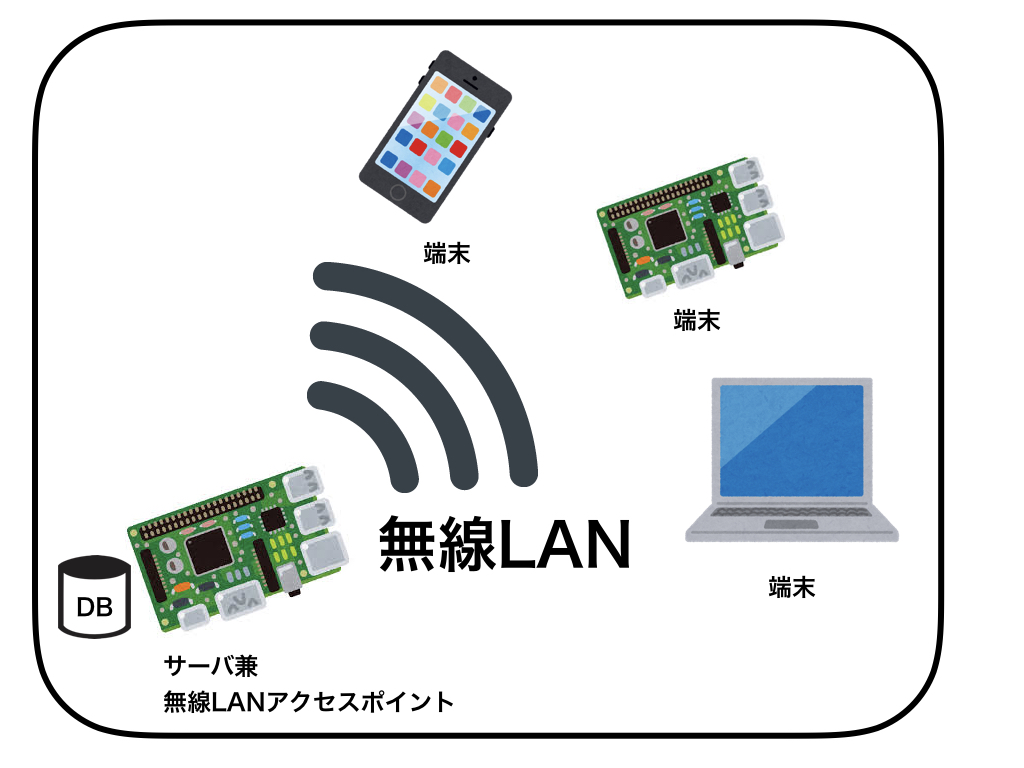
\includegraphics[width=1\linewidth,clip]{./wifi.jpeg}
    \caption{ログイン画面のイメージ図}\label{fig:wifi.jpeg}
  \end{center}
\end{figure}
